\subsection{Experiment One: Best Input Combination}

\subsubsection{Best Input Combination Results}
\label{sec:simpleInputTest}
The simple input test based on 3 month historical data and 200 epochs.

WS = Wind Speed
AD = Air Density
C = Consumption
T = Temperature
WD = Wind Direction
L-P = Last Known Production
D = Date
ToD = Time of Day
M = Time of Day as matrix

\footnotesize
\begin{center}
\begin{longtable}{|c|c|c|c|c|c|c|c|c|c|c|c|}
\caption{Wind Production Input Parameter Test}\\
\hline
\textbf{WS} & \textbf{AD} & \textbf{C} & \textbf{T} & \textbf{WD} & \textbf{L-P} & \textbf{D}& \textbf{ToD} & \textbf{MAE} & \textbf{\% from \#1} & \textbf{H1} & \textbf{H2} \\
\hline
\endfirsthead
\multicolumn{12}{c}%
{\tablename\ \thetable\ -- \textit{Continued from previous page}} \\
\hline
\textbf{WS} & \textbf{AD} & \textbf{C} & \textbf{T} & \textbf{WD} & \textbf{L-P} & \textbf{D}& \textbf{ToD} & \textbf{MAE} & \textbf{\% from \#1} & \textbf{H1} & \textbf{H2}  \\
\hline
\endhead
\hline \multicolumn{12}{r}{\textit{Continued on next page}} \\
\endfoot
\hline
\endlastfoot
\arrayrulecolor{light-gray}
 \x &  &  &  \x &  &  \x &  &  \x & 127,86 & 0,0\% & 19 & 13  \\ \hline
 \x &  \x &  &  &  \x &  \x &  &  \x & 131,59 & 2,92\% & 20 & 17  \\ \hline
 \x &  \x &  &  &  &  \x &  &  \x & 131,89 & 3,15\% & 16 & 20  \\ \hline
 \x &  \x &  \x &  \x &  \x &  \x &  &  \x & 133,18 & 4,16\% & 13 & 20  \\ \hline
 \x &  \x &  \x &  \x &  \x &  \x &  &  & 133,77 & 4,62\% & 16 & 17  \\ \hline
 \x &  \x &  \x &  &  &  \x &  &  \x & 134,14 & 4,91\% & 12 & 17  \\ \hline
 \x &  \x &  \x &  &  \x &  \x &  &  \x & 135,4 & 5,9\% & 6 & 13  \\ \hline
 \x &  \x &  \x &  &  &  \x &  &  & 136,33 & 6,62\% & 21 & 10  \\ \hline
 \x &  \x &  &  &  &  \x &  \x &  \x & 136,65 & 6,87\% & 5 & 24  \\ \hline
 \x &  &  &  &  &  \x &  &  & 137,33 & 7,41\% & 9 & 15  \\ \hline
 \x &  &  &  \x &  \x &  \x &  &  \x & 137,8 & 7,77\% & 17 & 16  \\ \hline
 \x &  \x &  &  &  \x &  \x &  &  & 138,16 & 8,06\% & 15 & 21  \\ \hline
 \x &  &  \x &  &  &  &  &  & 138,33 & 8,19\% & 23 & 13  \\ \hline
 \x &  \x &  &  \x &  &  \x &  &  & 138,94 & 8,67\% & 10 & 25  \\ \hline
 \x &  \x &  &  &  &  &  &  \x & 139,25 & 8,91\% & 23 & 12  \\ \hline
 \x &  \x &  &  &  &  \x &  &  & 139,35 & 8,99\% & 16 & 14  \\ \hline
 \x &  \x &  \x &  &  &  &  &  & 139,67 & 9,24\% & 17 & 20  \\ \hline
 \x &  &  \x &  &  \x &  \x &  &  \x & 139,78 & 9,32\% & 21 & 90  \\ \hline
 \x &  \x &  \x &  \x &  &  &  &  & 139,99 & 9,49\% & 11 & 19  \\ \hline
 \x &  &  &  &  &  &  &  \x & 140,14 & 9,6\% & 16 & 90  \\ \hline
 \x &  &  &  &  \x &  &  &  \x & 140,44 & 9,84\% & 17 & 20  \\ \hline
 \x &  &  &  \x &  &  \x &  &  & 140,55 & 9,92\% & 13 & 13  \\ \hline
 \x &  &  \x &  &  &  \x &  &  & 140,82 & 10,14\% & 18 & 16  \\ \hline
 \x &  \x &  \x &  &  &  &  &  \x & 140,85 & 10,16\% & 16 & 18  \\ \hline
 \x &  \x &  \x &  \x &  &  \x &  &  \x & 140,91 & 10,21\% & 18 & 13  \\ \hline
 \x &  \x &  &  &  &  &  &  & 141,09 & 10,35\% & 23 & 90  \\ \hline
 \x &  &  \x &  &  &  &  &  \x & 141,28 & 10,5\% & 19 & 15  \\ \hline
 \x &  &  \x &  &  \x &  &  &  \x & 141,38 & 10,57\% & 16 & 22  \\ \hline
 \x &  &  &  &  \x &  &  &  & 141,5 & 10,67\% & 18 & 10  \\ \hline
 \x &  &  &  &  \x &  \x &  &  & 142,22 & 11,23\% & 21 & 90  \\ \hline
 \x &  \x &  \x &  \x &  &  \x &  \x &  \x & 142,35 & 11,33\% & 5 & 20  \\ \hline
 \x &  \x &  &  \x &  \x &  &  &  \x & 142,44 & 11,4\% & 2 & 23  \\ \hline
 \x &  \x &  \x &  &  &  \x &  \x &  \x & 142,57 & 11,5\% & 15 & 14  \\ \hline
 \x &  \x &  &  \x &  &  \x &  &  \x & 142,64 & 11,56\% & 17 & 20  \\ \hline
 \x &  &  \x &  &  &  \x &  &  \x & 142,67 & 11,58\% & 18 & 13  \\ \hline
 \x &  \x &  \x &  &  \x &  &  &  & 142,75 & 11,65\% & 18 & 18  \\ \hline
 \x &  &  \x &  \x &  \x &  \x &  &  \x & 142,97 & 11,82\% & 25 & 12  \\ \hline
 \x &  \x &  &  &  \x &  &  &  \x & 143,07 & 11,9\% & 2 & 24  \\ \hline
 \x &  \x &  \x &  &  &  &  \x &  \x & 143,23 & 12,02\% & 6 & 25  \\ \hline
 \x &  &  \x &  \x &  &  \x &  &  \x & 143,24 & 12,03\% & 20 & 90  \\ \hline
 \x &  \x &  &  \x &  &  &  &  \x & 143,53 & 12,26\% & 21 & 10  \\ \hline
 \x &  \x &  &  &  \x &  &  &  & 143,98 & 12,61\% & 17 & 14  \\ \hline
 \x &  \x &  \x &  &  \x &  &  &  \x & 144,06 & 12,67\% & 12 & 21  \\ \hline
 \x &  \x &  \x &  &  &  \x &  \x &  & 144,24 & 12,81\% & 25 & 10  \\ \hline
 \x &  &  &  \x &  \x &  \x &  &  & 144,95 & 13,37\% & 12 & 20  \\ \hline
 \x &  \x &  \x &  &  \x &  \x &  &  & 144,96 & 13,37\% & 9 & 18  \\ \hline
 \x &  &  &  &  &  \x &  &  \x & 145,11 & 13,49\% & 18 & 13  \\ \hline
 \x &  \x &  &  \x &  \x &  \x &  &  & 145,26 & 13,61\% & 16 & 19  \\ \hline
 \x &  \x &  \x &  \x &  &  &  &  \x & 145,49 & 13,79\% & 2 & 23  \\ \hline
 \x &  &  \x &  &  \x &  \x &  \x &  & 145,92 & 14,12\% & 9 & 22  \\ \hline
 \x &  &  \x &  &  \x &  &  \x &  \x & 145,98 & 14,17\% & 11 & 18  \\ \hline
 \x &  &  \x &  &  &  &  \x &  \x & 146,02 & 14,2\% & 16 & 16  \\ \hline
 \x &  \x &  \x &  \x &  &  &  \x &  \x & 146,32 & 14,44\% & 16 & 90  \\ \hline
 \x &  &  \x &  \x &  &  &  &  \x & 146,48 & 14,56\% & 20 & 17  \\ \hline
 \x &  &  \x &  &  \x &  &  &  & 146,82 & 14,83\% & 15 & 19  \\ \hline
 \x &  \x &  &  &  &  &  \x &  \x & 147,08 & 15,03\% & 1 & 25  \\ \hline
 \x &  &  &  \x &  &  &  &  & 147,41 & 15,29\% & 21 & 10  \\ \hline
 \x &  \x &  &  \x &  \x &  \x &  \x &  \x & 147,99 & 15,74\% & 15 & 19  \\ \hline
 \x &  \x &  \x &  \x &  &  \x &  \x &  & 148,27 & 15,96\% & 20 & 10  \\ \hline
 \x &  &  \x &  \x &  \x &  \x &  &  & 148,61 & 16,23\% & 24 & 10  \\ \hline
 \x &  &  &  \x &  \x &  &  &  \x & 148,67 & 16,28\% & 13 & 22  \\ \hline
 \x &  &  &  \x &  &  &  &  \x & 149,27 & 16,74\% & 14 & 19  \\ \hline
 \x &  &  &  &  &  &  &  & 149,72 & 17,1\% & 9 & 25  \\ \hline
 \x &  &  \x &  &  &  &  \x &  & 149,8 & 17,16\% & 22 & 14  \\ \hline
 \x &  \x &  \x &  \x &  &  \x &  &  & 149,85 & 17,2\% & 25 & 10  \\ \hline
 \x &  &  &  &  &  \x &  \x &  \x & 150,3 & 17,55\% & 13 & 20  \\ \hline
 \x &  \x &  \x &  \x &  &  &  \x &  & 150,45 & 17,67\% & 22 & 16  \\ \hline
 \x &  &  \x &  \x &  \x &  &  &  & 150,63 & 17,81\% & 14 & 24  \\ \hline
 \x &  &  \x &  \x &  &  \x &  &  & 150,96 & 18,07\% & 14 & 13  \\ \hline
 \x &  &  \x &  &  \x &  \x &  &  & 151,54 & 18,52\% & 14 & 18  \\ \hline
 \x &  &  &  &  \x &  \x &  &  \x & 151,55 & 18,53\% & 21 & 90  \\ \hline
 \x &  &  \x &  &  &  \x &  \x &  \x & 151,92 & 18,82\% & 16 & 12  \\ \hline
 \x &  \x &  &  &  \x &  \x &  \x &  & 152,61 & 19,36\% & 2 & 18  \\ \hline
 \x &  \x &  \x &  &  \x &  &  \x &  & 152,89 & 19,58\% & 22 & 13  \\ \hline
 \x &  \x &  &  &  &  &  \x &  & 153,3 & 19,9\% & 13 & 13  \\ \hline
 \x &  \x &  &  &  \x &  &  \x &  & 153,31 & 19,9\% & 7 & 19  \\ \hline
 \x &  &  &  &  &  &  \x &  & 153,92 & 20,38\% & 22 & 90  \\ \hline
 \x &  &  \x &  \x &  &  &  &  & 154,02 & 20,46\% & 13 & 19  \\ \hline
 \x &  \x &  \x &  \x &  \x &  &  &  \x & 154,25 & 20,64\% & 9 & 24  \\ \hline
 \x &  \x &  \x &  &  \x &  &  \x &  \x & 154,51 & 20,84\% & 1 & 11  \\ \hline
 \x &  &  &  &  \x &  &  \x &  & 154,58 & 20,9\% & 7 & 22  \\ \hline
 \x &  \x &  &  &  &  \x &  \x &  & 154,85 & 21,11\% & 5 & 12  \\ \hline
 \x &  \x &  &  \x &  &  &  \x &  & 154,97 & 21,2\% & 15 & 15  \\ \hline
 \x &  \x &  &  \x &  \x &  &  \x &  \x & 155,07 & 21,28\% & 13 & 15  \\ \hline
 \x &  \x &  &  \x &  &  &  \x &  \x & 155,55 & 21,66\% & 1 & 25  \\ \hline
 \x &  &  &  &  \x &  &  \x &  \x & 156,13 & 22,11\% & 22 & 19  \\ \hline
 \x &  \x &  \x &  \x &  \x &  &  &  & 156,26 & 22,21\% & 15 & 21  \\ \hline
 \x &  &  \x &  \x &  &  &  \x &  \x & 156,52 & 22,42\% & 21 & 10  \\ \hline
 \x &  &  \x &  \x &  \x &  &  \x &  & 156,72 & 22,57\% & 9 & 23  \\ \hline
 \x &  \x &  &  \x &  \x &  &  &  & 156,94 & 22,74\% & 20 & 13  \\ \hline
 \x &  &  \x &  &  &  \x &  \x &  & 157,19 & 22,94\% & 7 & 22  \\ \hline
 \x &  &  &  &  &  &  \x &  \x & 157,36 & 23,07\% & 20 & 11  \\ \hline
 \x &  &  \x &  \x &  \x &  &  &  \x & 157,44 & 23,13\% & 15 & 16  \\ \hline
 \x &  \x &  &  &  \x &  &  \x &  \x & 157,56 & 23,23\% & 9 & 18  \\ \hline
 \x &  \x &  \x &  &  &  &  \x &  & 157,71 & 23,35\% & 24 & 90  \\ \hline
 \x &  &  &  \x &  \x &  &  \x &  & 158,06 & 23,62\% & 23 & 14  \\ \hline
 \x &  \x &  &  \x &  &  &  &  & 158,3 & 23,81\% & 19 & 14  \\ \hline
 \x &  &  &  \x &  &  &  \x &  \x & 158,4 & 23,89\% & 15 & 19  \\ \hline
 \x &  &  &  &  &  \x &  \x &  & 158,51 & 23,97\% & 13 & 16  \\ \hline
 \x &  \x &  \x &  \x &  \x &  &  \x &  \x & 159,52 & 24,76\% & 15 & 14  \\ \hline
 \x &  &  \x &  \x &  &  &  \x &  & 159,55 & 24,78\% & 19 & 19  \\ \hline
 \x &  &  \x &  \x &  \x &  &  \x &  \x & 160,37 & 25,43\% & 13 & 21  \\ \hline
 \x &  \x &  &  \x &  \x &  \x &  &  \x & 160,53 & 25,55\% & 16 & 20  \\ \hline
 \x &  &  &  &  \x &  \x &  \x &  \x & 160,56 & 25,57\% & 5 & 19  \\ \hline
 \x &  \x &  \x &  \x &  \x &  \x &  \x &  & 160,62 & 25,62\% & 18 & 14  \\ \hline
 \x &  &  \x &  \x &  \x &  \x &  \x &  & 161,1 & 26,0\% & 18 & 17  \\ \hline
 \x &  &  &  \x &  \x &  &  &  & 161,21 & 26,08\% & 21 & 15  \\ \hline
 \x &  &  \x &  &  \x &  \x &  \x &  \x & 161,23 & 26,1\% & 20 & 14  \\ \hline
 \x &  &  \x &  &  \x &  &  \x &  & 161,32 & 26,17\% & 21 & 14  \\ \hline
 \x &  &  &  \x &  \x &  &  \x &  \x & 165,26 & 29,25\% & 24 & 11  \\ \hline
 \x &  &  &  \x &  \x &  \x &  \x &  & 166,87 & 30,51\% & 1 & 16  \\ \hline
 \x &  &  &  \x &  &  \x &  \x &  & 167,74 & 31,19\% & 9 & 22  \\ \hline
 \x &  &  &  \x &  &  &  \x &  & 167,83 & 31,26\% & 17 & 17  \\ \hline
 \x &  \x &  &  \x &  \x &  \x &  \x &  & 168,73 & 31,96\% & 13 & 21  \\ \hline
 \x &  \x &  &  \x &  \x &  &  \x &  & 168,81 & 32,03\% & 17 & 15  \\ \hline
 \x &  \x &  \x &  &  \x &  \x &  \x &  \x & 169,41 & 32,5\% & 3 & 21  \\ \hline
 \x &  \x &  \x &  \x &  \x &  &  \x &  & 169,83 & 32,82\% & 12 & 21  \\ \hline
 \x &  &  &  \x &  \x &  \x &  \x &  \x & 169,92 & 32,9\% & 21 & 13  \\ \hline
 \x &  \x &  &  \x &  &  \x &  \x &  & 170,93 & 33,69\% & 9 & 18  \\ \hline
 \x &  &  \x &  \x &  \x &  \x &  \x &  \x & 171,61 & 34,22\% & 9 & 13  \\ \hline
 \x &  &  \x &  \x &  &  \x &  \x &  & 172,72 & 35,09\% & 14 & 15  \\ \hline
 \x &  &  &  &  \x &  \x &  \x &  & 173,12 & 35,4\% & 18 & 90  \\ \hline
 \x &  &  \x &  \x &  &  \x &  \x &  \x & 173,65 & 35,81\% & 13 & 17  \\ \hline
 \x &  \x &  \x &  \x &  \x &  \x &  \x &  \x & 174,26 & 36,29\% & 15 & 14  \\ \hline
 \x &  \x &  &  \x &  &  \x &  \x &  \x & 174,55 & 36,52\% & 3 & 17  \\ \hline
 \x &  &  &  \x &  &  \x &  \x &  \x & 174,85 & 36,75\% & 1 & 17  \\ \hline
 \x &  \x &  \x &  &  \x &  \x &  \x &  & 180,89 & 41,48\% & 20 & 11  \\ \hline
 \x &  \x &  &  &  \x &  \x &  \x &  \x & 199,22 & 55,81\% & 18 & 19  \\ \hline
\end{longtable}
\label{table:windProdInputParams}
\end{center}
\normalsize

\subsubsection{Best Input Combination Prediction Graphs}
\label{sec:bestCombiPredictionsGraphs}
The best prediction graphs for the input combination experiment.

\begin{sidewaysfigure}[h!]
\centering
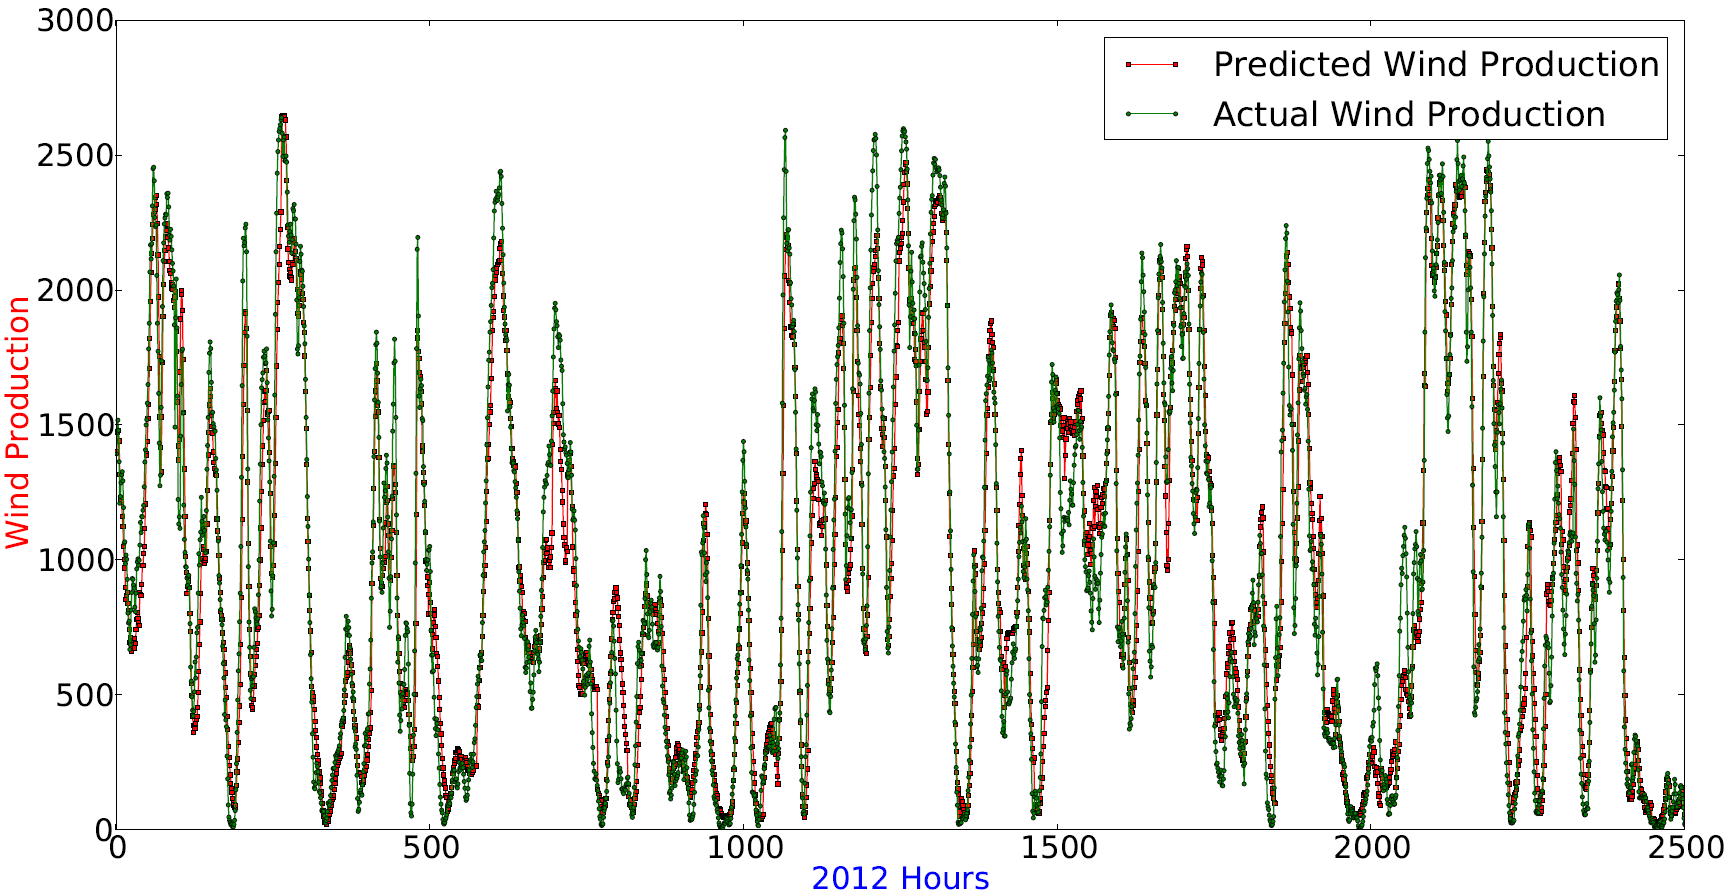
\includegraphics[width=0.99\linewidth]{billeder/bestInputCombi0-2500.png}
\caption{Wind Power prediction for 0-2500 hours in 2012 with the best combination}
\label{fig:bestInputCombi0-2500}
\end{sidewaysfigure} 

\begin{sidewaysfigure}[h!]
\centering
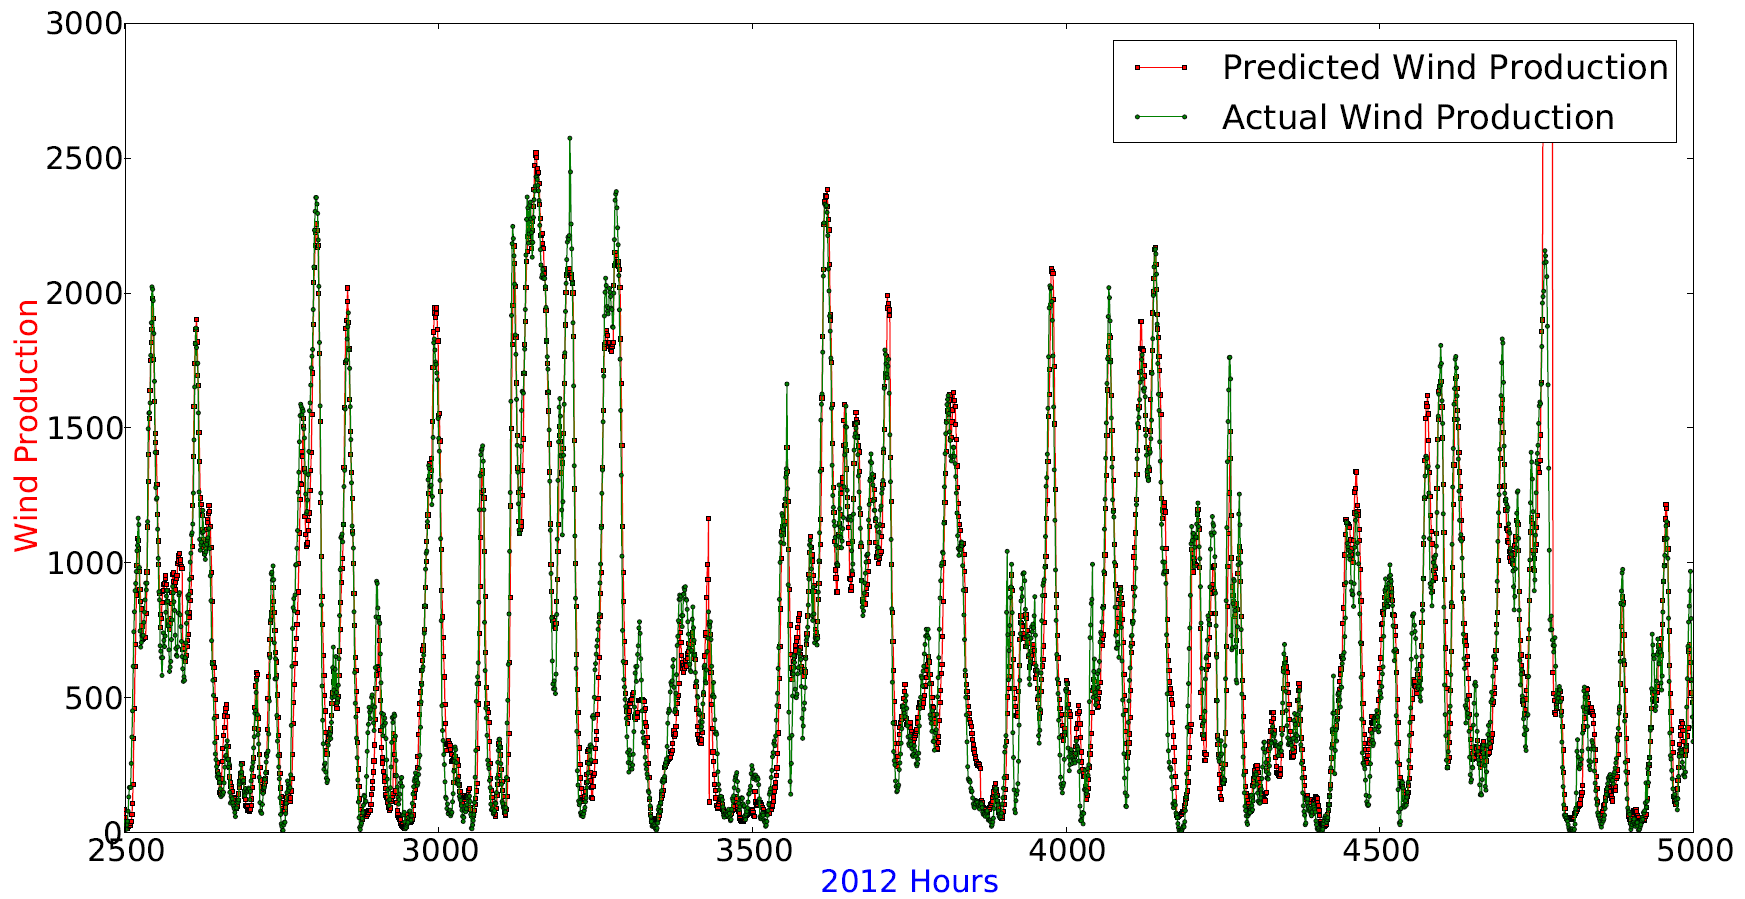
\includegraphics[width=0.99\linewidth]{billeder/bestInputCombi2500-5000.png}
\caption{Wind Power prediction for 2500-5000 hours in 2012 with the best combination}
\label{fig:bestInputCombi2500-5000}
\end{sidewaysfigure} 

\subsection{Experiment Two:}

\subsubsection{Simple input test with seasonality}
\label{sec:simpleInputTestSeason}
The simple input test based on 3 months before the prediction day and the same month in the previous year. All with 200 epochs.

WS = Wind Speed
AD = Air Density
C = Consumption
T = Temperature
WD = Wind Direction
L-P = Last Known Production
D = Date
ToD = Time of Day
M = Time of Day as matrix

\footnotesize
\begin{center}
\begin{longtable}{|c|c|c|c|c|c|c|c|c|c|c|c|}
\caption{Wind Production Input Parameter Test}\\
\hline
\textbf{WS} & \textbf{AD} & \textbf{C} & \textbf{T} & \textbf{WD} & \textbf{L-P} & \textbf{D}& \textbf{ToD} & \textbf{MAE} & \textbf{\% from \#1} & \textbf{H1} & \textbf{H2} \\
\hline
\endfirsthead
\multicolumn{10}{c}%
{\tablename\ \thetable\ -- \textit{Continued from previous page}} \\
\hline
\textbf{WS} & \textbf{AD} & \textbf{C} & \textbf{T} & \textbf{WD} & \textbf{L-P} & \textbf{D}& \textbf{ToD} & \textbf{MAE} & \textbf{\% from \#1} & \textbf{H1} & \textbf{H2} \\
\hline
\endhead
\hline \multicolumn{10}{r}{\textit{Continued on next page}} \\
\endfoot
\hline
\endlastfoot
\arrayrulecolor{light-gray}
 \x &  \x &  \x &  &  \x &  \x &  &  \x & 142.88 & 0.0\% & 7 & 17 \\ \hline
 \x &  &  &  \x &  \x &  \x &  &  & 142.89 & 0.01\% & 14 & 11 \\ \hline
 \x &  \x &  &  &  \x &  \x &  &  \x & 143.37 & 0.34\% & 3 & 21 \\ \hline
 \x &  \x &  \x &  \x &  \x &  \x &  &  \x & 143.97 & 0.76\% & 4 & 25 \\ \hline
 \x &  &  &  &  &  \x &  &  \x & 143.98 & 0.77\% & 2 & 21 \\ \hline
 \x &  \x &  \x &  \x &  &  \x &  \x &  & 144.11 & 0.86\% & 1 & 17 \\ \hline
 \x &  \x &  &  &  &  \x &  &  & 144.12 & 0.87\% & 7 & 12 \\ \hline
 \x &  &  &  &  &  &  &  \x & 144.28 & 0.98\% & 12 & 17 \\ \hline
 \x &  &  \x &  &  \x &  \x &  &  & 144.42 & 1.08\% & 11 & 10 \\ \hline
 \x &  \x &  &  \x &  \x &  \x &  &  \x & 144.48 & 1.12\% & 1 & 17 \\ \hline
 \x &  &  \x &  \x &  &  \x &  &  & 144.7 & 1.27\% & 21 & 60 \\ \hline
 \x &  \x &  \x &  \x &  &  \x &  &  & 144.79 & 1.34\% & 18 & 13 \\ \hline
 \x &  &  &  &  &  \x &  &  & 144.93 & 1.43\% & 18 & 10 \\ \hline
 \x &  &  \x &  \x &  \x &  \x &  \x &  & 144.98 & 1.47\% & 14 & 90 \\ \hline
 \x &  &  \x &  \x &  &  \x &  \x &  & 145.02 & 1.5\% & 18 & 11 \\ \hline
 \x &  \x &  \x &  \x &  &  \x &  \x &  \x & 145.19 & 1.62\% & 2 & 15 \\ \hline
 \x &  &  &  \x &  &  \x &  \x &  & 145.29 & 1.69\% & 13 & 60 \\ \hline
 \x &  \x &  &  &  &  &  &  \x & 145.51 & 1.84\% & 1 & 22 \\ \hline
 \x &  &  \x &  &  \x &  \x &  &  \x & 145.76 & 2.02\% & 13 & 17 \\ \hline
 \x &  \x &  \x &  &  \x &  &  &  \x & 145.79 & 2.04\% & 18 & 90 \\ \hline
 \x &  \x &  \x &  &  \x &  \x &  \x &  & 145.98 & 2.17\% & 1 & 90 \\ \hline
 \x &  &  \x &  &  &  &  &  & 145.99 & 2.18\% & 16 & 13 \\ \hline
 \x &  &  &  &  \x &  &  &  & 146.24 & 2.35\% & 24 & 90 \\ \hline
 \x &  \x &  \x &  &  \x &  \x &  &  & 146.49 & 2.53\% & 2 & 13 \\ \hline
 \x &  &  \x &  &  &  \x &  &  \x & 146.53 & 2.55\% & 1 & 18 \\ \hline
 \x &  \x &  \x &  &  &  &  &  & 146.57 & 2.58\% & 24 & 11 \\ \hline
 \x &  \x &  \x &  &  \x &  \x &  \x &  \x & 146.61 & 2.61\% & 5 & 15 \\ \hline
 \x &  \x &  &  \x &  \x &  \x &  \x &  & 146.64 & 2.63\% & 1 & 13 \\ \hline
 \x &  \x &  \x &  \x &  \x &  \x &  \x &  \x & 146.78 & 2.73\% & 4 & 16 \\ \hline
 \x &  \x &  \x &  \x &  \x &  \x &  \x &  & 146.89 & 2.81\% & 4 & 16 \\ \hline
 \x &  \x &  &  &  &  &  &  & 146.96 & 2.86\% & 25 & 50 \\ \hline
 \x &  \x &  \x &  &  &  \x &  &  & 147.18 & 3.01\% & 14 & 15 \\ \hline
 \x &  &  \x &  \x &  &  \x &  &  \x & 147.3 & 3.09\% & 17 & 70 \\ \hline
 \x &  &  &  &  &  \x &  \x &  \x & 147.64 & 3.33\% & 11 & 11 \\ \hline
 \x &  &  \x &  &  &  &  &  \x & 147.7 & 3.37\% & 11 & 22 \\ \hline
 \x &  \x &  \x &  &  &  &  &  \x & 147.86 & 3.49\% & 10 & 25 \\ \hline
 \x &  &  &  &  \x &  \x &  \x &  \x & 147.95 & 3.55\% & 4 & 17 \\ \hline
 \x &  &  \x &  &  &  \x &  &  & 147.98 & 3.57\% & 14 & 17 \\ \hline
 \x &  &  &  &  \x &  \x &  \x &  & 148.23 & 3.74\% & 1 & 23 \\ \hline
 \x &  \x &  &  \x &  &  \x &  \x &  \x & 148.28 & 3.78\% & 5 & 13 \\ \hline
 \x &  &  &  \x &  \x &  \x &  \x &  & 148.4 & 3.86\% & 13 & 13 \\ \hline
 \x &  \x &  &  \x &  &  \x &  &  & 148.57 & 3.98\% & 21 & 14 \\ \hline
 \x &  \x &  \x &  \x &  &  &  &  \x & 148.66 & 4.05\% & 14 & 20 \\ \hline
 \x &  \x &  \x &  \x &  &  &  &  & 149.0 & 4.28\% & 7 & 25 \\ \hline
 \x &  \x &  &  &  \x &  &  &  \x & 149.04 & 4.31\% & 16 & 12 \\ \hline
 \x &  &  &  \x &  &  \x &  &  & 149.08 & 4.34\% & 19 & 15 \\ \hline
 \x &  &  \x &  &  &  \x &  \x &  & 149.13 & 4.37\% & 3 & 16 \\ \hline
 \x &  \x &  \x &  &  &  \x &  \x &  \x & 149.28 & 4.48\% & 2 & 16 \\ \hline
 \x &  \x &  &  \x &  \x &  \x &  &  & 149.31 & 4.5\% & 1 & 17 \\ \hline
 \x &  &  \x &  &  \x &  &  &  \x & 149.4 & 4.56\% & 14 & 18 \\ \hline
 \x &  \x &  \x &  &  &  \x &  &  \x & 149.95 & 4.95\% & 1 & 16 \\ \hline
 \x &  &  \x &  &  \x &  \x &  \x &  & 150.28 & 5.18\% & 1 & 22 \\ \hline
 \x &  \x &  \x &  \x &  &  \x &  &  \x & 150.33 & 5.21\% & 9 & 19 \\ \hline
 \x &  \x &  &  &  &  \x &  \x &  \x & 150.36 & 5.24\% & 4 & 15 \\ \hline
 \x &  \x &  &  &  &  \x &  &  \x & 150.98 & 5.67\% & 21 & 10 \\ \hline
 \x &  &  &  &  \x &  &  &  \x & 151.09 & 5.75\% & 11 & 21 \\ \hline
 \x &  &  \x &  \x &  &  &  &  & 151.13 & 5.77\% & 20 & 10 \\ \hline
 \x &  &  &  \x &  &  &  &  \x & 151.3 & 5.89\% & 20 & 15 \\ \hline
 \x &  \x &  &  \x &  &  \x &  &  \x & 151.45 & 6.0\% & 7 & 20 \\ \hline
 \x &  \x &  \x &  \x &  \x &  \x &  &  & 151.46 & 6.01\% & 10 & 24 \\ \hline
 \x &  \x &  &  &  \x &  \x &  \x &  \x & 151.48 & 6.02\% & 2 & 16 \\ \hline
 \x &  \x &  &  \x &  \x &  \x &  \x &  \x & 151.67 & 6.15\% & 4 & 17 \\ \hline
 \x &  &  \x &  \x &  &  &  &  \x & 151.7 & 6.17\% & 17 & 13 \\ \hline
 \x &  &  \x &  \x &  \x &  \x &  \x &  \x & 151.76 & 6.22\% & 2 & 16 \\ \hline
 \x &  &  \x &  \x &  \x &  \x &  &  \x & 151.91 & 6.32\% & 1 & 90 \\ \hline
 \x &  &  \x &  \x &  &  \x &  \x &  \x & 152.06 & 6.42\% & 7 & 22 \\ \hline
 \x &  \x &  &  &  \x &  &  &  & 152.25 & 6.56\% & 19 & 12 \\ \hline
 \x &  &  &  &  \x &  \x &  &  \x & 152.28 & 6.58\% & 19 & 14 \\ \hline
 \x &  \x &  &  \x &  &  &  &  \x & 152.35 & 6.63\% & 23 & 12 \\ \hline
 \x &  \x &  &  &  &  \x &  \x &  & 152.36 & 6.63\% & 10 & 22 \\ \hline
 \x &  \x &  \x &  \x &  \x &  &  \x &  \x & 152.39 & 6.66\% & 18 & 90 \\ \hline
 \x &  &  &  \x &  \x &  \x &  &  \x & 152.43 & 6.68\% & 6 & 23 \\ \hline
 \x &  \x &  &  &  \x &  \x &  &  & 153.17 & 7.2\% & 2 & 10 \\ \hline
 \x &  \x &  \x &  &  &  &  \x &  & 153.2 & 7.22\% & 7 & 13 \\ \hline
 \x &  &  \x &  \x &  \x &  &  \x &  \x & 153.3 & 7.29\% & 13 & 20 \\ \hline
 \x &  &  \x &  \x &  &  &  \x &  & 153.52 & 7.45\% & 16 & 15 \\ \hline
 \x &  &  &  \x &  &  &  &  & 153.6 & 7.5\% & 22 & 14 \\ \hline
 \x &  \x &  \x &  &  &  \x &  \x &  & 153.82 & 7.66\% & 8 & 14 \\ \hline
 \x &  &  \x &  \x &  \x &  &  &  & 153.84 & 7.67\% & 9 & 20 \\ \hline
 \x &  &  &  &  \x &  \x &  &  & 153.95 & 7.75\% & 15 & 12 \\ \hline
 \x &  &  \x &  &  \x &  &  &  & 154.16 & 7.89\% & 14 & 13 \\ \hline
 \x &  \x &  &  \x &  &  &  &  & 154.18 & 7.91\% & 12 & 24 \\ \hline
 \x &  \x &  \x &  \x &  &  &  \x &  & 154.84 & 8.37\% & 13 & 18 \\ \hline
 \x &  &  &  \x &  \x &  \x &  \x &  \x & 154.94 & 8.44\% & 1 & 18 \\ \hline
 \x &  \x &  \x &  \x &  &  &  \x &  \x & 154.95 & 8.45\% & 2 & 21 \\ \hline
 \x &  \x &  &  \x &  &  &  \x &  & 155.0 & 8.48\% & 18 & 12 \\ \hline
 \x &  &  &  &  &  &  &  & 155.07 & 8.53\% & 7 & 21 \\ \hline
 \x &  \x &  \x &  &  \x &  &  \x &  & 155.46 & 8.8\% & 16 & 15 \\ \hline
 \x &  &  \x &  \x &  \x &  &  \x &  & 155.7 & 8.97\% & 16 & 18 \\ \hline
 \x &  \x &  \x &  \x &  \x &  &  &  \x & 155.79 & 9.04\% & 19 & 11 \\ \hline
 \x &  \x &  \x &  &  &  &  \x &  \x & 155.82 & 9.06\% & 7 & 22 \\ \hline
 \x &  &  \x &  \x &  &  &  \x &  \x & 155.89 & 9.11\% & 13 & 22 \\ \hline
 \x &  \x &  &  &  &  &  \x &  & 156.04 & 9.21\% & 22 & 80 \\ \hline
 \x &  &  &  \x &  &  \x &  &  \x & 156.14 & 9.28\% & 1 & 21 \\ \hline
 \x &  \x &  &  &  \x &  &  \x &  \x & 156.34 & 9.42\% & 14 & 16 \\ \hline
 \x &  &  &  \x &  \x &  &  \x &  \x & 156.59 & 9.6\% & 12 & 22 \\ \hline
 \x &  &  &  &  &  \x &  \x &  & 156.6 & 9.6\% & 22 & 10 \\ \hline
 \x &  &  \x &  &  \x &  \x &  \x &  \x & 156.84 & 9.77\% & 1 & 10 \\ \hline
 \x &  &  \x &  &  &  &  \x &  & 156.89 & 9.81\% & 14 & 19 \\ \hline
 \x &  \x &  &  \x &  \x &  &  \x &  \x & 157.48 & 10.22\% & 12 & 17 \\ \hline
 \x &  &  &  \x &  &  &  \x &  & 157.61 & 10.31\% & 15 & 14 \\ \hline
 \x &  &  &  \x &  \x &  &  &  \x & 158.37 & 10.84\% & 25 & 90 \\ \hline
 \x &  \x &  &  &  \x &  &  \x &  & 158.46 & 10.9\% & 5 & 23 \\ \hline
 \x &  \x &  &  \x &  \x &  &  &  \x & 158.64 & 11.03\% & 22 & 90 \\ \hline
 \x &  \x &  &  &  &  &  \x &  \x & 158.74 & 11.1\% & 24 & 10 \\ \hline
 \x &  \x &  &  &  \x &  \x &  \x &  & 159.01 & 11.29\% & 2 & 23 \\ \hline
 \x &  &  \x &  &  \x &  &  \x &  \x & 159.25 & 11.46\% & 12 & 23 \\ \hline
 \x &  \x &  \x &  \x &  \x &  &  \x &  & 159.32 & 11.51\% & 14 & 24 \\ \hline
 \x &  \x &  \x &  &  \x &  &  \x &  \x & 159.44 & 11.59\% & 14 & 12 \\ \hline
 \x &  &  \x &  &  &  \x &  \x &  \x & 159.6 & 11.7\% & 2 & 13 \\ \hline
 \x &  \x &  \x &  &  \x &  &  &  & 159.74 & 11.8\% & 12 & 14 \\ \hline
 \x &  &  &  \x &  &  &  \x &  \x & 159.94 & 11.94\% & 11 & 15 \\ \hline
 \x &  \x &  &  \x &  &  \x &  \x &  & 160.11 & 12.06\% & 10 & 14 \\ \hline
 \x &  \x &  \x &  \x &  \x &  &  &  & 160.55 & 12.37\% & 15 & 19 \\ \hline
 \x &  &  &  &  \x &  &  \x &  \x & 160.79 & 12.53\% & 17 & 13 \\ \hline
 \x &  &  &  &  &  &  \x &  & 160.98 & 12.67\% & 10 & 21 \\ \hline
 \x &  \x &  &  \x &  \x &  &  \x &  & 161.12 & 12.77\% & 13 & 13 \\ \hline
 \x &  &  &  &  &  &  \x &  \x & 161.18 & 12.81\% & 18 & 12 \\ \hline
 \x &  &  \x &  &  &  &  \x &  \x & 161.25 & 12.86\% & 3 & 25 \\ \hline
 \x &  &  \x &  \x &  \x &  &  &  \x & 161.5 & 13.03\% & 18 & 17 \\ \hline
 \x &  &  &  &  \x &  &  \x &  & 161.59 & 13.09\% & 16 & 20 \\ \hline
 \x &  \x &  &  \x &  &  &  \x &  \x & 162.1 & 13.45\% & 6 & 22 \\ \hline
 \x &  &  \x &  &  \x &  &  \x &  & 162.54 & 13.76\% & 12 & 13 \\ \hline
 \x &  \x &  &  \x &  \x &  &  &  & 162.55 & 13.77\% & 19 & 15 \\ \hline
 \x &  &  &  \x &  &  \x &  \x &  \x & 162.57 & 13.78\% & 4 & 23 \\ \hline
 \x &  &  &  \x &  \x &  &  &  & 162.87 & 13.99\% & 15 & 19 \\ \hline
 \x &  &  &  \x &  \x &  &  \x &  & 163.34 & 14.32\% & 15 & 19 \\ \hline
 \x &  &  \x &  \x &  \x &  \x &  &  & 165.37 & 15.74\% & 13 & 18 \\ \hline
\end{longtable}
\label{table:windProdInputParamsSeasonal}
\end{center}
\normalsize

\subsubsection{Historical volatility results}
\label{sec:historicalVolatiltiyResultsAppendix}
Historical volatility results with all combinations of previous hours between 4-24 and different smoothing factors.

\footnotesize
\begin{center}
\begin{longtable}{|c|c|c|c|}
\caption{Wind Production Input Parameter Test}\\
\hline
\textbf{Previous Hours} & \textbf{Smoothing factor} & \textbf{MAE} & \textbf{\% Deviation} \\
\hline
\endfirsthead
\multicolumn{4}{c}%
{\tablename\ \thetable\ -- \textit{Continued from previous page}} \\
\hline
\textbf{Previous Hours} & \textbf{Smoothing factor} & \textbf{MAE} & \textbf{\% Deviation} \\
\hline
\endhead
\hline \multicolumn{4}{r}{\textit{Continued on next page}} \\
\endfoot
\hline
\endlastfoot
\arrayrulecolor{light-gray}
6 & 0,70 & 121,81 & 0,0\% \\ \hline
20 & 0,80 & 122,9 & 0,89\% \\ \hline
24 & 0,60 & 123,13 & 1,08\% \\ \hline
24 & 0,80 & 124,02 & 1,81\% \\ \hline
16 & 0,20 & 125,65 & 3,15\% \\ \hline
12 & 0,30 & 127,0 & 4,26\% \\ \hline
24 & 0,70 & 127,06 & 4,31\% \\ \hline
16 & 0, 60 & 127,38 & 4,57\% \\ \hline
24 & 0,40 & 127,51 & 4,68\% \\ \hline
16 & 0,90 & 127,77 & 4,89\% \\ \hline
16 & 0,30 & 127,86 & 4,97\% \\ \hline
4 & 0,60 & 128,49 & 5,48\% \\ \hline
4 & 0,10 & 128,51 & 5,5\% \\ \hline
20 & 0,50 & 129,36 & 6,2\% \\ \hline
8 & 0,10 & 130,06 & 6,77\% \\ \hline
24 & 0,20 & 131,05 & 7,59\% \\ \hline
12 & 0,90 & 131,87 & 8,26\% \\ \hline
20 & 0,10 & 132,63 & 8,88\% \\ \hline
20 & 0,30 & 133,32 & 9,45\% \\ \hline
6 & 0,20 & 133,67 & 9,74\% \\ \hline
4 & 0,30 & 133,84 & 9,88\% \\ \hline
12 & 0,60 & 134,02 & 10,02\% \\ \hline
4 & 0,20 & 134,18 & 10,16\% \\ \hline
16 & 0,40 & 134,28 & 10,24\% \\ \hline
4 & 0,40 & 134,71 & 10,59\% \\ \hline
12 & 0,40 & 135,05 & 10,87\% \\ \hline
16 & 0,80 & 135,14 & 10,94\% \\ \hline
20 & 0,20 & 135,3 & 11,07\% \\ \hline
12 & 0,50 & 135,42 & 11,17\% \\ \hline
24 & 0,90 & 135,71 & 11,41\% \\ \hline
16 & 0,50 & 136,44 & 12,01\% \\ \hline
4 & 0,50 & 136,58 & 12,13\% \\ \hline
6 & 0,30 & 136,6 & 12,14\% \\ \hline
20 & 0,70 & 136,63 & 12,17\% \\ \hline
20 & 0,60 & 136,86 & 12,36\% \\ \hline
12 & 0,20 & 136,98 & 12,45\% \\ \hline
6 & 0,10 & 137,16 & 12,6\% \\ \hline
24 & 0,10 & 137,34 & 12,75\% \\ \hline
6 & 0,50 & 137,45 & 12,84\% \\ \hline
24 & 0,50 & 137,91 & 13,22\% \\ \hline
20 & 0,90 & 137,92 & 13,23\% \\ \hline
8 & 0,20 & 138,26 & 13,5\% \\ \hline
8 & 0,40 & 138,69 & 13,86\% \\ \hline
6 & 0,60 & 138,87 & 14,01\% \\ \hline
8 & 0,50 & 138,93 & 14,05\% \\ \hline
8 & 0,60 & 139,2 & 14,28\% \\ \hline
8 & 0,90 & 139,84 & 14,8\% \\ \hline
8 & 0,70 & 140,01 & 14,94\% \\ \hline
24 & 0,30 & 140,45 & 15,3\% \\ \hline
6 & 0,70 & 141,3 & 16,0\% \\ \hline
8 & 0,30 & 141,6 & 16,25\% \\ \hline
4 & 0,70 & 142,19 & 16,73\% \\ \hline
12 & 0,80 & 142,2 & 16,74\% \\ \hline
6 & 0,40 & 142,98 & 17,38\% \\ \hline
6 & 0,80 & 143,21 & 17,57\% \\ \hline
20 & 0,40 & 143,59 & 17,88\% \\ \hline
8 & 0,80 & 143,62 & 17,9\% \\ \hline
12 & 0,10 & 144,37 & 18,52\% \\ \hline
16 & 0,70 & 144,43 & 18,57\% \\ \hline
16 & 0,10 & 146,77 & 20,49\% \\ \hline
4 & 0,80 & 146,9 & 20,6\% \\ \hline
6 & 0,90 & 147,48 & 21,07\% \\ \hline
4 & 0,90 & 151,15 & 24,09\% \\ \hline
\end{longtable}
\label{table:historicalVolatilityAppendixTable}
\end{center}
\normalsize